\setlength{\columnsep}{3pt}
\begin{flushleft}
	
	\begin{itemize}
		\item The partition table in MBR can hold only \textbf{4 entries}.
		\item Hence, there can be only \textbf{four partitions in hard disks}.
		\item These 4 partitions are called primary partitions.
		\item OS can be installed on the primary partition.
		\begin{figure}[h!]
			\centering
			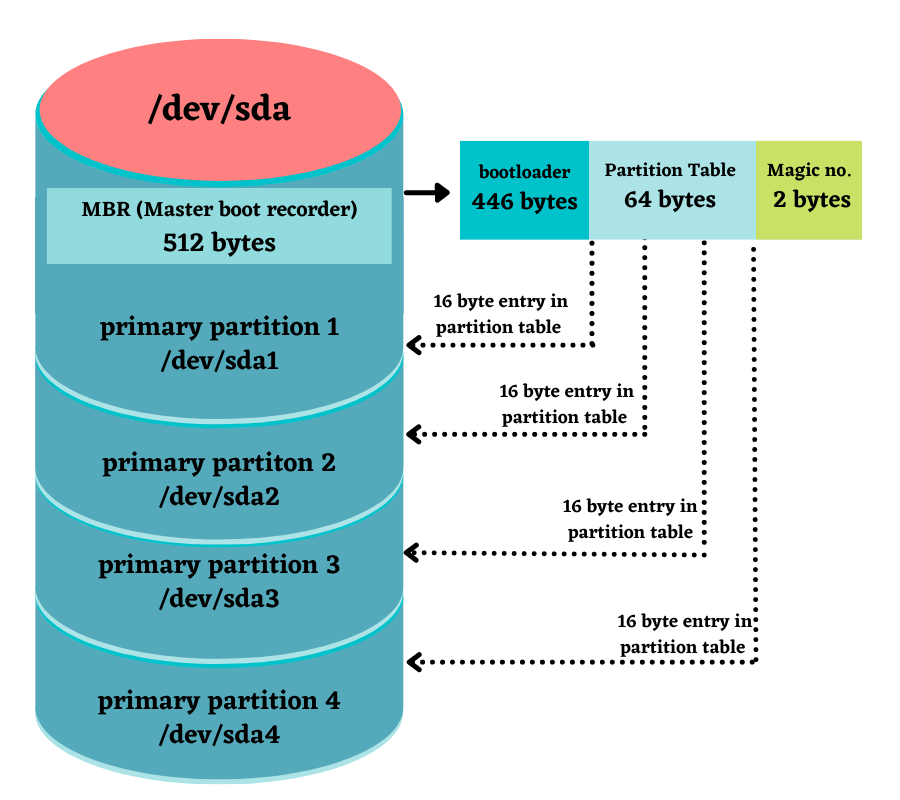
\includegraphics[scale=.6]{content/chapter8/images/correct.png}
			\caption{Primary partitions}
			\label{primary_naming}
		\end{figure}		
		
	\end{itemize}

\newpage

\paragraph{Command to create primary partition}

\bigskip
\textbf{fdisk}: Used to change the partition table.
	\bigskip
	\begin{tcolorbox}[breakable,notitle,boxrule=-0pt,colback=pink,colframe=pink]
		\color{black}
		\fontdimen2\font=9pt
		Syntax: fdisk device\_name
		\fontdimen2\font=4pt
	\end{tcolorbox}

	Options for \textbf{fdisk} command:
	\begin{itemize}
		\item \textbf{p}: Print the partition table
		\item \textbf{n}: Create a new partition
		\item \textbf{w}: Write the new partition table and exit
	\end{itemize}

	Eg:
	\begin{figure}[h!]
		\centering
		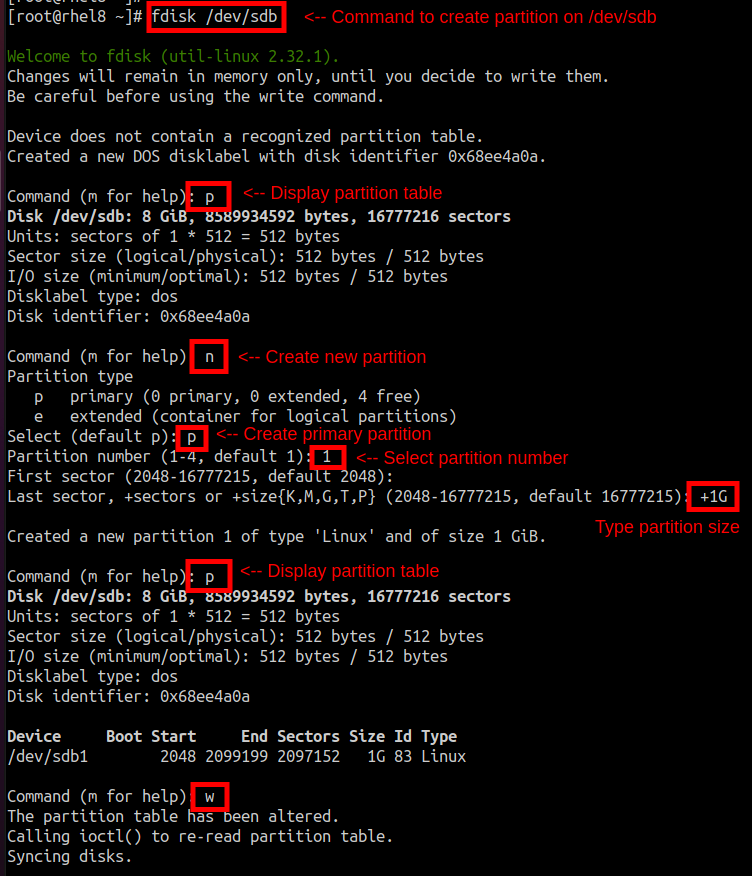
\includegraphics[scale=.4]{content/chapter8/images/primary_fdisk.png}
		\caption{Creating primary partitions}
		\label{pp}
	\end{figure}		
			
	
\end{flushleft}

\newpage

